
\chapter{WISDEM Floating Turbine Analysis}
\label{sec:other}
Direct WISDEM dependencies to \textit{CommonSE} and \textit{TowerSE}, as well as some of the
supporting utilities housed under the WISDEM umbrella, were mentioned in
Section \ref{sec:package}.  There are other inputs into \textit{FloatingSE} that
are outputs of other WISDEM modules.  For example force, moment, and
mass properties of the RNA.  An OpenMDAO Group that links these other
modules together to form a virtual floating turbine does not explicitly
fit within the conceptual boundaries of the \texttt{src/floatingse} package.
However, two files within the \textit{WISDEM} module (meant for
high-level coupling of multiple WISDEM components) \texttt{src/floating}-directory
do assemble the virtual floating turbine,

{\small
\begin{tabularx}{\textwidth}{ l X }
\texttt{floating\_turbine\_assembly.py} & OpenMDAO Group that connects  multiple WISDEM modules for a complete floating offshore turbine simulation and optimization.\\
\texttt{floating\_turbine\_instance.py} & Implements the above assembly
and extends.
\end{tabularx}
}

The WISDEM modules that exchange inputs and outputs within this
high-level assembly to crteate a virtual floating wind turbine are
listed in Table \ref{tbl:new_wisdem}.  In addition to
\textit{FloatingSE}, two other new WISDEM modules are also required to
fully represent a floating offshore wind plant (beyond just a single
turbine), \textit{OffshoreBOS\_SE} and \textit{Offshore\_OandM\_SE}.
With these two additions, WISDEM can be diagrammed as shown in Figure
\ref{fig:new_wisdem}.  While the core development of
\textit{OffshoreBOS\_SE} is effectively complete,
\textit{Offshore\_OandM\_SE} has not yet been implemented. Note that as
of this writing, \textit{DriveSE} is not yet connected to the others,
but doing so is part of the near-term development plan.

\begin{table}[htbp] \begin{center}
    \caption{WISDEM modules that comprise a virtual floating offshore
      wind plant.}
    \label{tbl:new_wisdem}
{\footnotesize
  \begin{tabularx}{\textwidth}{ l X } \hline
    \textbf{Module} & \textbf{Description} \\
\textit{RotorSE} & Analysis of aerodynamic and structural loading of rotor
  blades, determination of turbine power curve, and calculation of
  annual energy production (AEP)\\
\textit{CommonSE} & Wind and wave velocity profiles, drag calculations,
  probabilities distributions, frustum and tubular mass properties, math
  utilities, structural code compliance checks, and RNA aggregator\\
\textit{OffshoreBOS\_SE} & Capital costs for wind plant items aside from the
  turbine, such as cabling and substations.  Assembly, installation,
  commissioning, decommissioning, and financing costs for all
  components. See \citep{obos}\\
\textit{FloatingSE} & Floating substructure, including mooring and anchors, and
  static stability calculations\\
\textit{TurbineCostsSE (2015)} & Capital costs for all turbine components
  above the water line\\
\textit{PlantFinanceSE} & Roll-up of capital costs, balance of station
  costs, operational costs, financing rates, and net energy production
  into the levelized cost of energy (LCOE)\\
\textit{DriveSE} & Analysis of drive shaft, bearings, and gearbox.  See
  \citep{DriveSE}. NOT YET IMPLEMENTED\\
\textit{Offshore\_OandM\_SE} & Operational and maintenance costs.  NOT YET
    DEVELOPED\\
  \hline \end{tabularx}
}
\end{center} \end{table}

\begin{figure}[htb]
  \begin{center}
    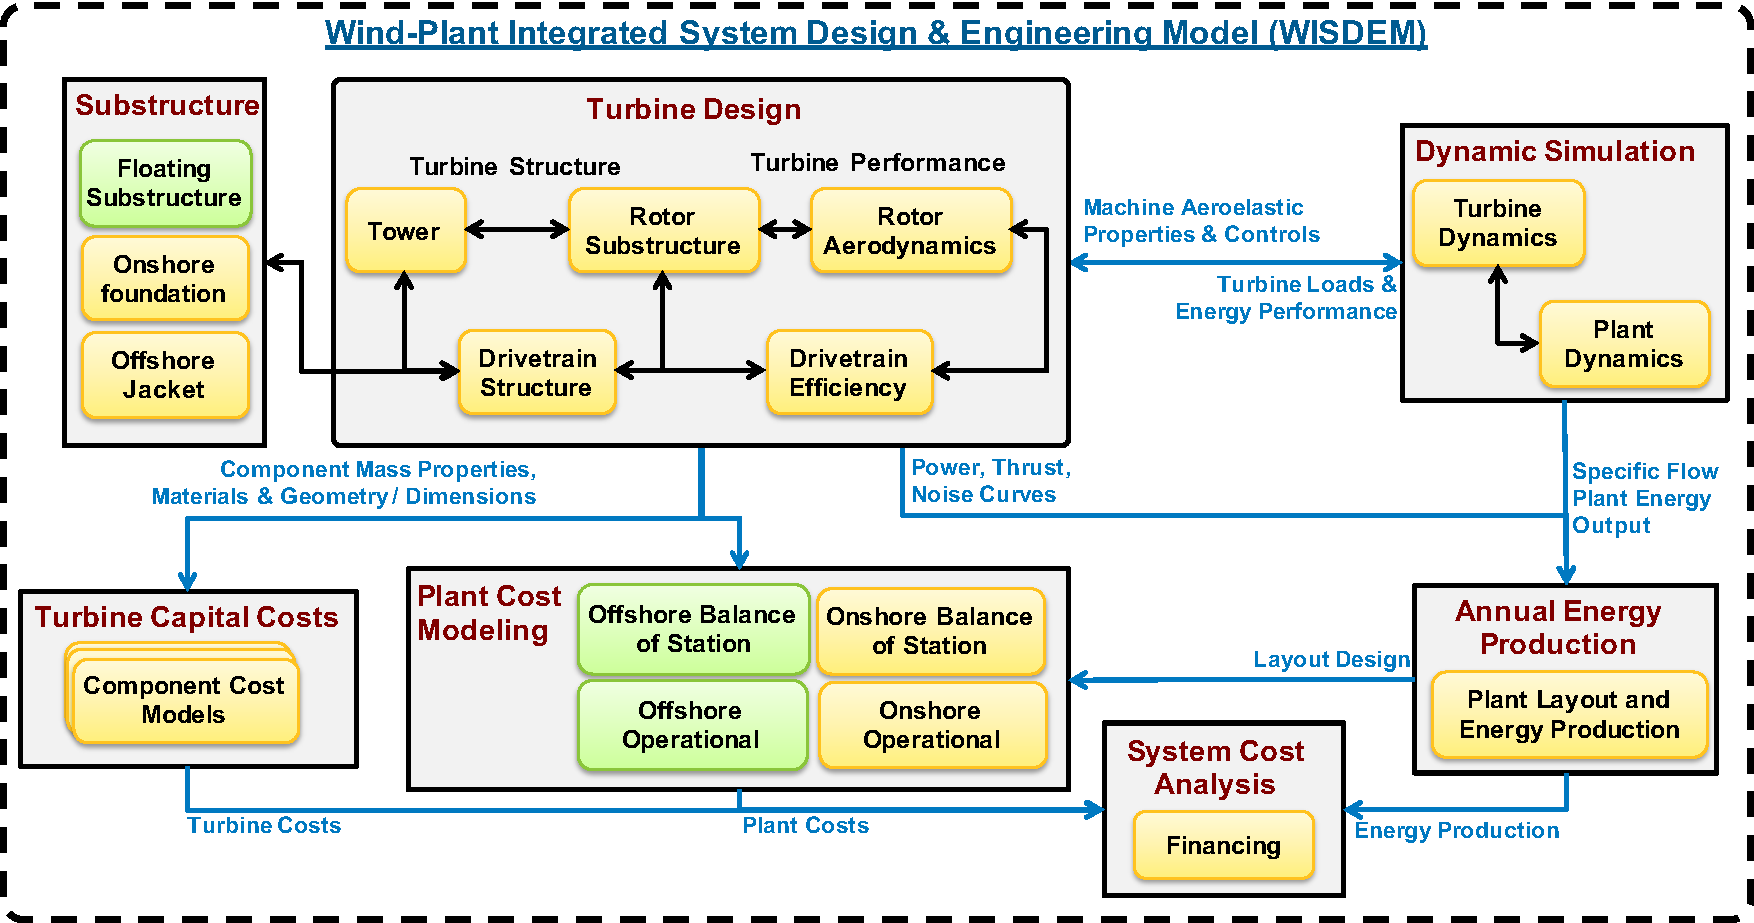
\includegraphics[width=6in]{figs/new_wisdem.pdf}
    \caption{Conceptual diagram of WISDEM following the addition of
      \textit{FloatingSE} and other modules (green boxes) to support offshore floating
      wind turbines.}
    \label{fig:new_wisdem}
  \end{center}
\end{figure}


With a floating offshore turbine constructed, system-wide optimization
and sensitivity studies can be conducted.  An obvious objective function
for these optimizations would be the levelized cost of energy (LCOE) as
output from the \textit{PlantFinanceSE} module.  This optimization would
require additional constraints pertinent to the other modules to produce
relevant results.  These other constraints are more suitably discussed
within the documentation of their home modules.  Depending on the nature
of the analysis, the user may wish to include other design variables in
the optimization that are inputs to one of these other modules.  As with
the constraints, the documentation of these design variables is best
found in their home modules.

%\section{Example}
%TODO

\begin{table}[htbp] \begin{center}
    \caption{Additional constraints used in full floating offshore
      turbine optimization.}
    \label{tbl:constraints-turb}
    {\footnotesize
  \begin{tabular}{ c l c l} \hline
    \textbf{Lower} & \textbf{Name} & \textbf{Upper} & \textbf{Description}\\
\hline \hline
    & \textbf{Rotor} &  &\\
 & rotor.P1\_margin & 1.00 & Blade frequency keep away from 1P rotor frequency\\
 & rotor.Pn\_margin & 1.00 & Blade frequency keep away from 3P rotor frequency\\
 & rotor.rotor\_buckling\_sparL & 1.00 & Rotor blade upper spar cap structural buckling unity constraint\\
 & rotor.rotor\_buckling\_sparU & 1.00 & Rotor blade lower spar cap structural buckling unity constraint\\
 & rotor.rotor\_buckling\_teL & 1.00 & Rotor blade upper trailing edge panel structural buckling unity constraint\\
 & rotor.rotor\_buckling\_teU & 1.00 & Rotor blade lower trailing edge panel structural buckling unity constraint\\
 & rotor.rotor\_damage\_sparL & 0.00 & Rotor blade upper spar cap structural damage constraint\\
 & rotor.rotor\_damage\_sparU & 0.00 & Rotor blade lower spar cap structural damage constraint\\
 & rotor.rotor\_damage\_teL & 0.00 & Rotor blade upper trailing edge panel structural damage constraint\\
 & rotor.rotor\_damage\_teU & 0.00 & Rotor blade lower trailing edge panel structural damage constraint\\
 & rotor.rotor\_strain\_sparL & 1.00 & Rotor blade upper spar cap structural strain unity constraint\\
  -1.00 & rotor.rotor\_strain\_sparU &  & Rotor blade lower spar cap structural strain unity constraint\\
 & rotor.rotor\_strain\_teL & 1.00 & Rotor blade upper trailing edge panel structural strain unity constraint\\
  -1.00 & rotor.rotor\_strain\_teU &  & Rotor blade lower trailing edge panel structural strain unity constraint\\
 & \textbf{Geometry} &  & \\
  20.00 & tcons.ground\_clearance &  & Minimum ground clearance of rotor blades\\
 & tcons.tip\_deflection\_ratio & 1.00 & Tip deflection limit to prevent tower strike as unity\\
 & \textbf{Stability} &  & \\
  1.00 & tcons.frequency1P\_margin\_high &  & Eigenfrequencies of entire structure must be below 1P frequency\\
 & tcons.frequency1P\_margin\_low & 1.00 & Eigenfrequencies of entire structure must be above 1P frequency\\
  1.00 & tcons.frequency3P\_margin\_high &  & Eigenfrequencies of entire structure must be below 3P frequency\\
 & tcons.frequency3P\_margin\_low & 1.00 & Eigenfrequencies of entire structure must be above 3P frequency\\
    \hline \end{tabular}
  }
\end{center} \end{table}
